\section{Potentiometer}

\subsection{Hysterese und Nichtlinearität}

Dieses Diagramm zeigt die Hysterese und die Nicht-linearität des Potentiometers im Bereich von 0 bis 20mm mit einer Schrittweite von 0.5mm.\\

\begin{figure}[H]
    \centering
    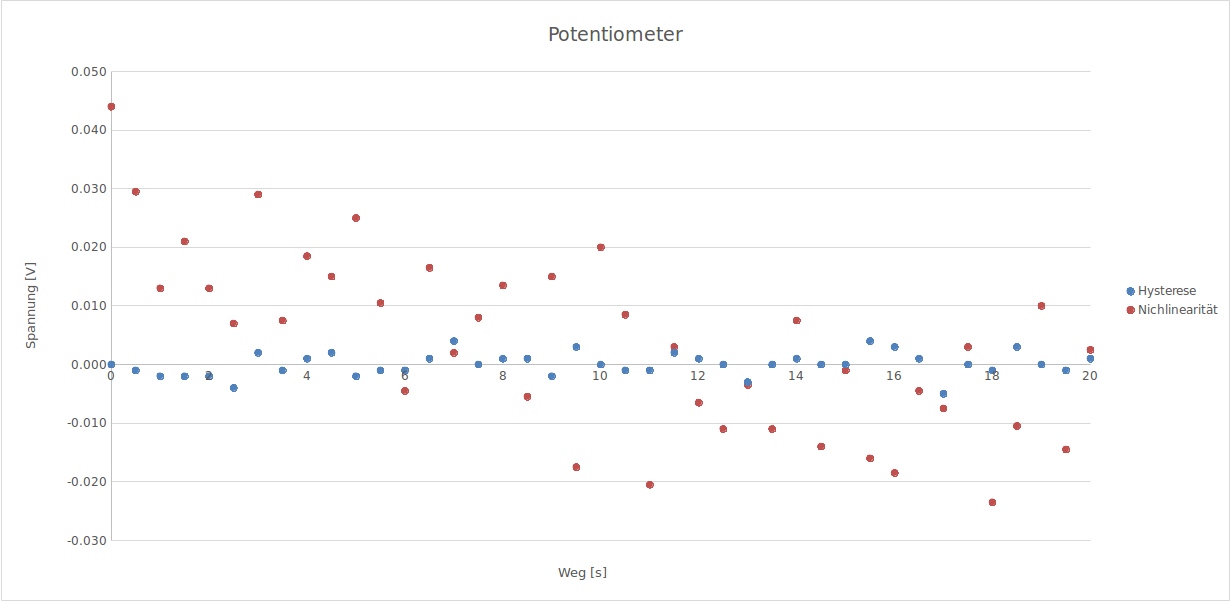
\includegraphics[scale=0.5]{pic/poti1.png}
    \caption{Potentiometrischer Sensor}
    \label{fig:poti}
\end{figure}

Eine Hysterese ist nicht erkennbar aus der Grafik. Die Abweichung gegenüber der Nominalspannung liegt innerhalb 5mV. Die enstspricht $\frac{5mV}{20 V} = 0.025\%$\\

Der Spannungsteiler wird von Potentiometer nicht signifikant belastet. Aus diesem Grund ist die Nicht-linearität sehr schwach ausgefallen.

\subsection{Berechnungen}


\begin{tabular}{ l  l }
    Max. Nicht-linearität: & $\varepsilon_L = \frac{|max(\epsilon_L)|}{|Messbereich|}
                                            = \frac{|45mV|}{|20V|}  
                                            = 0.225\%                             $  \\
    Max. Hysterese:        & $\varepsilon_H = \frac{|max(\epsilon_H)|}{|Messbereich|}
                                            = \frac{|5mV|}{|20V|} 
                                            = 0.025\%                             $  \\
\end{tabular}


\clearpage